% https://tex.stackexchange.com/questions/65544/how-to-link-table-of-contents-in-thesis-pdf
\cleardoublepage
\phantomsection
\renewcommand\contentsname{Table of Contents}
%\pdfbookmark[section]{\contentsname}{Table of Contents}
\addcontentsline{toc}{chapter}{Table of Contents}
\tableofcontents
\cleardoublepage
\phantomsection

\iffalse
\addcontentsline{toc}{chapter}{List of Todos}
\listoftodos
\cleardoublepage
\phantomsection
\fi

\addcontentsline{toc}{chapter}{List of Tables}
\listoftables
\cleardoublepage
\phantomsection

\addcontentsline{toc}{chapter}{List of Figures}
\listoffigures
\cleardoublepage
\phantomsection

\addcontentsline{toc}{chapter}{List of Theorems}
\listoftheorems[ignoreall,show={theorem,lemma}]
\cleardoublepage
\phantomsection

\chapter*{Mathematical Conventions}
\addcontentsline{toc}{chapter}{Mathematical Conventions}
\label{typography}

This thesis follows standard mathematical conventions of using lower-case italic variables~($u(t)$) to represent scalar quantities, lower-case bold variables~($\V{x}(t)$) to represent vector quantities, upper-case italic variables~($A$) to represent matrices, and Greek letters~($\tau$, $\theta$) to represent quantities with a unit of time.
Bars are included above variables ($\bar{A}$) to indicate that it has been discretized in time.
Depending on context, $F(s)$ or $F(z)$ are used to represent complex values in the Laplace $s$-domain, or $z$-domain, respectively.

\cleardoublepage
\phantomsection

\begin{figure}
\centering
\vspace*{\fill}
\begingroup
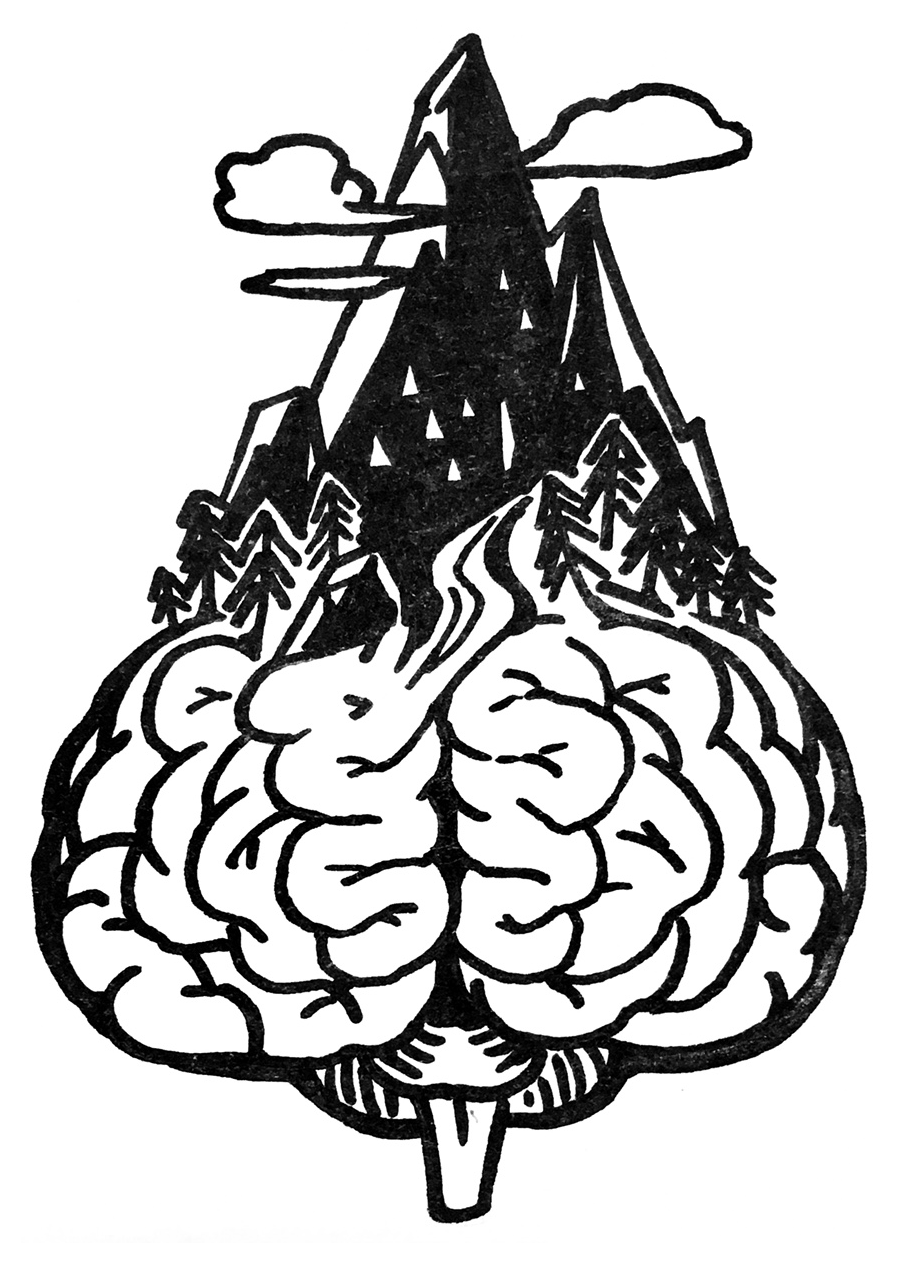
\includegraphics[width=0.6\columnwidth]{yang-peng-telluride-back-2018.png}
\endgroup

\vspace{1em} 

\begin{CJK*}{UTF8}{gbsn}
愚公移山
\end{CJK*}
\vspace*{\fill}
\end{figure}

\cleardoublepage
\phantomsection

% Change page numbering back to Arabic numerals
\pagenumbering{arabic}
